\chapter{Effects of Patient-Specific Variability in Inconsistent End-Expiratory Diaphragm Position On the Quantification of Left Ventricular Cardiac Strains}

\textit{Adapted from...}

\section{Synopsis}
	\noindent \textbf{Purpose:}  To determine if normal inconsistency in end-expiratory diaphragm position between separate image acquisitions significantly affects estimates of cardiac strains.

	\noindent \textbf{Materials and Methods:} We enrolled 17 subjects, including seven patients with heart disease. For each subject, we measured the range of end-expiratory positions during 10 separate breath-holds. The imaging protocol comprised two ventricular long-axis and three short-axis slices of navigator-gated 2D cine displacement encoding with stimulated echoes (DENSE) cardiac magnetic resonance (MR). To simulate end-expiratory position inconsistency, DENSE images were each acquired at the patient-specific minimum, middle, and maximum end-expiratory positions; a repeated acquisition at the middle position was used to quantify variability independent of end-expiratory differences. Differences and variability of left ventricular peak strains were compared using analysis of variance and Student’s t-test.
	
	\noindent \textbf{Results:} The range of end-expiratory positions across 10~breath-holds was 10~$\pm$~4~mm. There were no significant differences in global or regional peak radial, circumferential, or longitudinal strains measured at the different end-expiratory positions (p~=~0.17–--0.98). In general, there were also no differences in variability in global or regional peak strains between inconsistent (minimum, middle, and maximum) and consistent (two acquisitions from middle position) end-expiratory positions (p~=~0.10--–0.95). With at least 80\% power, the study had an ability to detect global differences of 4.7\%, 1.0\%, and 1.7\% (absolute) between end-expiratory positions for radial, circumferential, and longitudinal strains, respectively.
	
	\noindent \textbf{Conclusion:} Measurements of left ventricular peak strains with DENSE cardiac MR are relatively insensitive to normal changes in end-expiratory position between separate image acquisitions.
	\bigskip
	
	\noindent \textbf{Keywords:} Cardiac Strains, Breath-holds, DENSE, Respiratory Navigator Gating
	
\newpage

\section{Background}
	Cardiac strains describe the deformation of myocardial tissue during contraction and relaxation. Measures of cardiac strains have been shown to be superior predictors of outcomes, such as mortality, compared to traditional measures of cardiac function or traditional clinical risk factors alone \cite{Stanton2009}. Imaging can non-invasively assess cardiac strains using echocardiographic techniques such as speckle tracking \cite{Amundsen2006} and cardiovascular magnetic resonance (MR) techniques such as myocardial feature tracking \cite{Hor2010}, myocardial tissue tagging \cite{Axel1989,Zerhouni1988}, phase velocity mapping \cite{Pelc1994}, strain encoding \cite{Osman2001}, and displacement encoding with stimulated echoes (DENSE) \cite{Aletras1999b,Aletras1999c}.

	Peak strains vary longitudinally throughout the left ventricle \cite{Kuijer2002,Moore2000,Young1994a,Feng2009,NasiraeiMoghaddam2010,Donekal2013a,Suever2017}. For example, previous studies have shown that left ventricular radial, circumferential, and longitudinal strains vary between the base and apex by up to 14\%, 5\%, and 5\% (absolute), respectively \cite{Kuijer2002,Moore2000,Young1994a,Feng2009,NasiraeiMoghaddam2010,Donekal2013a,Suever2017}. Cardiac MR images are often acquired during end-expiratory breath-holds to minimize respiratory motion artifacts. However, it is often difficult to achieve consistency in end-expiratory diaphragm position between successive breath holds, and variations of 4 to 13 mm are normal [17–21] \cite{Liu1993,Wang1995a,Taylor1997a,Holland1998c,Fischer2006a}. Inconsistent end-expiratory positions will impact the position of the heart with respect to the imaging plane (Figure~\ref{fig:diaphragmTranslation}). For example, previous studies have reported short-axis and long-axis through-plane displacements of up to 14 mm due to displacement of diaphragm position between breath-holds \cite{Slomka2007,Swingen2003}, and other studies have reported that the superior/inferior position of the heart can displace 55-92\% of the displacement of the diaphragm position \cite{Wang1995b,McLeish2002}. Because peak strains vary throughout the left ventricle, we hypothesize that translation of the heart with respect to the imaging plane to result in differences and variability in measured strains.

	To our knowledge, no study has evaluated the sensitivity of cardiac strains to natural end-expiratory position variability. This is an important knowledge gap, especially since the use of cardiac strains is increasing dramatically both in research and clinical practice. The purpose of this study was to determine if normal inconsistency in end-expiratory position significantly affects the quantification of cardiac strains and therefore results in higher variability in measured cardiac strains compared to strains measured at a consistent end-expiratory position.
	
	\begin{figure} 
		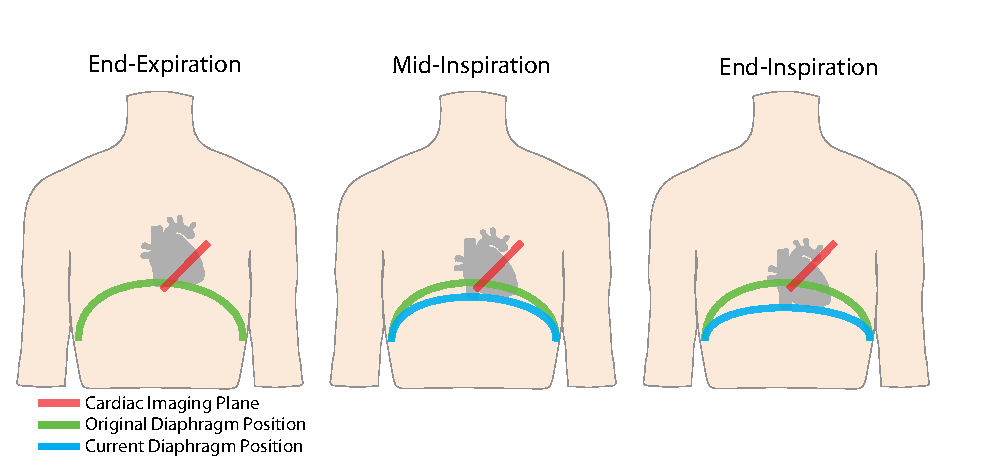
\includegraphics{figures/strainpaper/Fig1-range_of_diaphragm_position_breathing}
		\caption[During respiration, diaphragm motion causes the heart to translate a significant distance while the imaging plane remains fixed]{\textbf{During respiration, diaphragm motion causes the heart to translate a significant distance while the imaging plane remains fixed.}}
		\label{fig:diaphragmTranslation}
	\end{figure}
	
	

